\input{../preamble.tex}

\SetDate[01/04/2026]

\begin{document}
\pagestyle{fancy}
\fancyhead[L]{Tle STMG}
\fancyhead[C]{\textbf{Fonction inverse}}
\fancyhead[R]{\today}


\exe{}{
	Considérons la fonction inverse
		\[ f(x) = \dfrac1x. \]
	Calculer l'image par $f$ des nombres suivants.
		\begin{multicols}{3}
		\begin{enumerate}
			\item 
			10
			\item
			$-1$
			\item
			$\frac27$
			\item
			$10^{130}$
			\item
			$10^{-130}$
			\item
			$-5^{34}$
		\end{enumerate}
		\end{multicols}
}{exe:images-inverse}{
	todo
}

\exe{}{
	Tracer la courbe représentative de la fonction inverse dans le repère figure \ref{fig:1}.
}{exe:graph}{
	todo
}

\begin{figure}[h!]
	\centering
	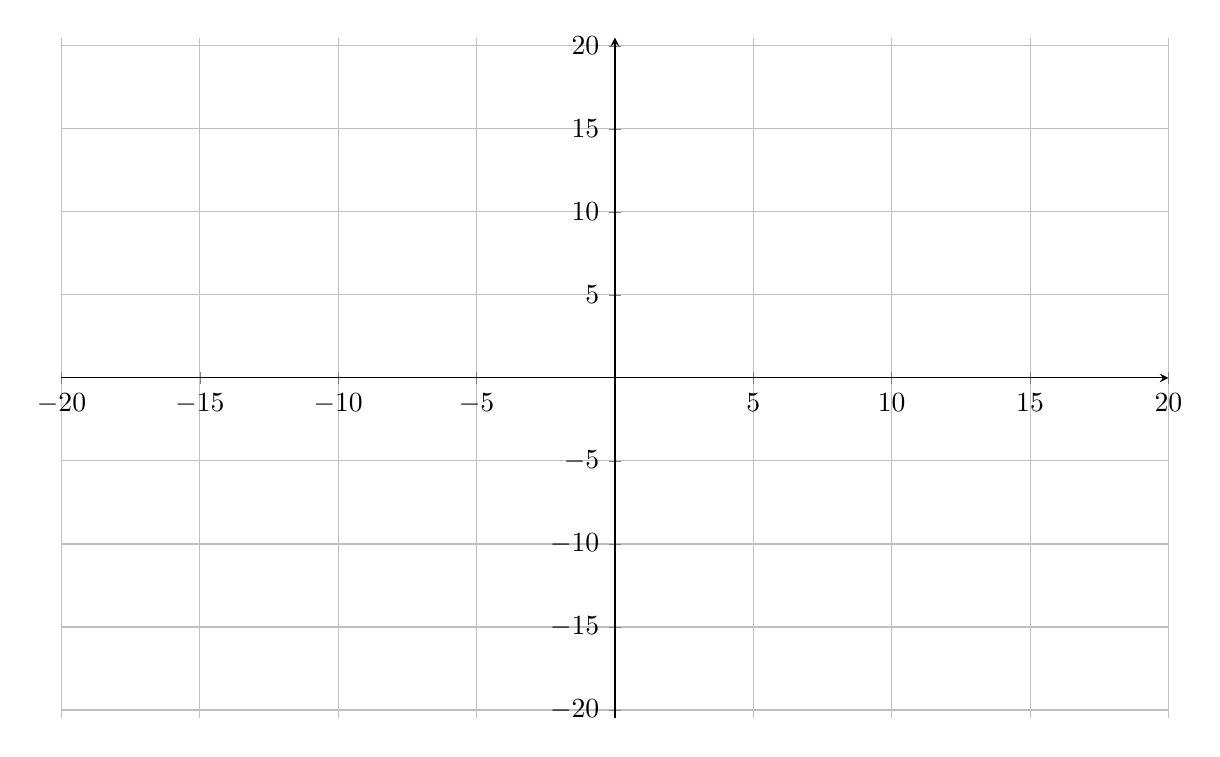
\begin{tikzpicture}[>=stealth]
		\begin{axis}[xmin = -20, xmax=20, ymin=-20.5, ymax=20.5, axis x line=middle, axis y line=middle, axis line style=->, grid=both, clip=true, x=10pt, y=6pt, extra x ticks = {}, ytick distance = 5, minor x tick num=0]
			\addplot[transparent, very thick, -, ] expression[domain=0:100, samples=1000]{log10(x)} node[pos=.5, above] {$\C_{\log}$};
		\end{axis}
	\end{tikzpicture}
	\caption{Repère de l'exercice \ref{exe:graph}.}
	\label{fig:1}
\end{figure}

\exe{}{
	Comparer les nombres suivants à l'aide de la courbe de la fonction inverse tracée figure \ref{fig:1}.
		\begin{multicols}{3}
		\begin{enumerate}[label=\roman*)]
			\item $\dfrac1{0,7}$ et $\dfrac1{2,5}$
			\item $\dfrac1{-2}$ et $\dfrac1{-3}$
			\item $\dfrac1{-4}$ et $\dfrac1{3}$
		\end{enumerate}
		\end{multicols}
}{exe:comparaisons}{
	todo
}

\exe{}{
	Trouver le nombre $x$ non nul vérifiant chaque équation.
	\begin{multicols}{4}
	\begin{enumerate}
		\item
		$\dfrac1x = 3$
		\item
		$\dfrac4x = 20$
		\item
		$\dfrac3x + 10 = 31$
		\item
		$\dfrac8x - 7 = \dfrac2x + 11$
	\end{enumerate}
	\end{multicols}
}{exe:eq-inv}{
	todo
}


%\exe{, difficulty=1}{
%Une entreprise produit des automates industriels. Elle décide d'estimer leur valeur à la vente selon la méthode suivante :
%\begin{enumerate}[label=(\roman*)]
%\item L'entreprise décompte les erreurs commises par les automates sur 1000 tâches. Elle note $x$ ce nombre d'erreurs.
%\item La valeur du robot est ensuite fixée en calculant le quotient $\frac{100~000}{x}$.
%\end{enumerate}
%\begin{enumerate}
%\item La valeur du robot décroît-elle en fonction de nombres d'erreurs commises ? Justifier.
%\item Existe-t-il un cas pour lequel cette méthode est problématique ? Justifier.
%\end{enumerate}
%}{exe:7}{
%
%}

%\newpage

\exe{,difficulty=1}{
	Une plateforme de comptabilité propose le tarif suivant :
		\begin{itemize}
			\item
			un coût initial de 90€ ; et
			\item
			un coût mensuel de 13€.
		\end{itemize}
	Un auto-entrepreneur étudie le prix du service comparé à celui de son comptable.
	\begin{enumerate}
		\item
		Quel prix doit-il payer pour 10 mois d'abonnement ?
		\item
		Donner le prix total à payer en fonction de $x$ où $x$ est le nombre de mois d'abonnement.
		\item
		Montrer que le prix mensuel $p(x)$ est donné par
			\[ p(x) = \frac{90}x + 13. \]
		\item
		Compléter le tableau de valeurs.
		
		\begin{center}
\def\arraystretch{2}
\setlength\tabcolsep{15pt}
		\begin{tabular}{|c|c|c|c|c|}\hline
			$x$ & 6 & 12 & 18 & 24 \\\hline
			$f(x)$ &&&& \\ \hline
		\end{tabular}
		\end{center}
		\item
		Le comptable facture ses services 256 euros par an.
		\begin{enumerate}
			\item
			Calculer le prix mensuel de ses services.
			\item
			Est-il plus avantageux d'utiliser la plateforme de comptabilité après 6 mois d'utilisation ? Et 12 mois ?
			\item
			À partir de combien de mois exactement la plateforme devient-elle plus avantageuse ?
		\end{enumerate}
	\end{enumerate}
}{exe:compatable}{
	todo
}




%\exe{}{
%	En course à pied, l'allure correspond au temps nécessaire (en minutes) pour parcourir 1 kilomètre.
%	Elle s'exprime donc en min/km.
%	
%	\begin{enumerate}
%		\item
%		Une femme a mis 18 minutes pour parcourir 3 kilomètres.
%			\begin{enumerate}
%				\item
%				Quelle est son allure en min/km ?
%				\item
%				Quelle est sa vitesse moyenne en km/min ?
%				\item
%				Comment passer de l'allure à la vitesse moyenne (km/min) ? et de la vitesse moyenne (km/min) à l'allure ?
%				\item
%				Quelle est sa vitesse moyenne en km/h ?
%			\end{enumerate}
%		\item
%		Si l'allure d'une personne est de 15 min/km, quelle est sa vitesse moyenne en km/h ?
%		\item
%		Si la vitesse d'une personne est de 8km/h, quelle est son allure en min/km ?
%	\end{enumerate}
%}{exe:allure}{
%
%}


\exe{, difficulty=1}{
	Une entreprise désire commercialiser un objet.
	Elle se fixe un objectif de résultat net de 200 000€.
		\begin{itemize}
			\item
			Les coûts de production fixes sont de 48 000€.
			\item
			Le coût de production d'un objet est de 5€ par unité.
		\end{itemize}
		\begin{enumerate}
			\item
			Supposons que 10 000 objets soient produits et vendus.
			\begin{enumerate}
				\item
				Donner le coût de production total.
				Celui-ci comprend les coûts fixes ainsi que ceux de production des objets.
				\item
				Combien d'argent doivent-ils gagner pour obtenir un résultat net de 200 000€ ?
				\item
				Quel prix de l'objet doit être fixé pour atteindre cet objectif ?
			\end{enumerate}
			\item
			Supposons désormais que $x$ objets soit produits et vendus.
			\begin{enumerate}
				\item
				Donner le coût de production total.
				Celui-ci comprend les coûts fixes ainsi que ceux de production des objets.
				\item
				Combien d'argent doivent-ils rapporter pour obtenir un résultat net de 200 000€ ?
				\item
				Quel prix de l'objet doit donc être fixé pour atteindre cet objectif ?
				Montrer qu'il est \mbox{égal à}
				\[ p(x) = \frac{248~000}{x} + 5. \]
			\end{enumerate}
			\item 
			Supposons que l'entreprise produise et vende 20 000 objets. Quel prix d'objet fixer pour atteindre l'objectif de bénéfices ?
			\item
			Combien d'objets doit l'entreprise produire et vendre pour que le prix fixé de l'objet soit égal à 9,99€ (prix psychologique) tout en atteignant son objectif de bénéfices ?
			\item 
			Supposons que l'entreprise dispose d'un marché illimité dans lequel elle peut vendre autant d'objets qu'elle le souhaite.
			Peut-elle baisser le prix de l'objet indéfiniment tout en atteignant son objectif de bénéfices fixé ?
		\end{enumerate}
}{exe:8}{

}




%%%%%%%%%%%%

\newpage
\fancyhead[C]{\textbf{Solutions}}
\shipoutAnswer

\end{document}
